
\documentclass{article}
\usepackage{graphicx}
\usepackage[french]{babel}
\usepackage{multicol}
\usepackage{geometry}
\usepackage{titling}
\usepackage[utf8]{inputenc}
\usepackage{natbib}
\usepackage[style=authoryear,backend=biber]{biblatex}
\usepackage{hyperref}
\usepackage{float}

\addbibresource{name.bib}

\geometry{
    a4paper,
    total={170mm,257mm},
    left=20mm,
    top=30mm,
}

\title{
    
\includegraphics[width=1\textwidth]{photo/UCLouvain_Charleroi.png} \\
    \vspace{1.5cm}
    {\Huge \textbf{Rapport Personnel \\ Projet Bite2Meet}} \\
    \vspace{1.5cm}
}

\author{
    \textbf{Moussaoui Noah} \\
    Université catholique de Louvain-la-Neuve \\
    Campus de Charleroi, EPL en SINC \\
    Délégué et ambassadeur \\
    \texttt{Noah.moussaoui@student.uclouvain.be}
}

\date{
    \vspace{1.5cm}
    Durée de recherche : Septembre - Novembre \\
    \vspace{1.5cm}
    
\includegraphics[width=0.5\textwidth]{photo/EPL.png}
}

\begin{document}

\maketitle
\newpage

\section{Introduction}
Dans ce projet, nous avons travaillé sur une application mobile innovante permettant 
aux utilisateurs qui sont des requins de rencontrer d'autres requins, mais sans adopter le format traditionnel des applications
de rencontres. Il s'agit d'un réseau social où les utilisateurs peuvent se retrouver pour 
chasser des humains , consulter des publications, découvrir des événements, 
et visionner des stories.\\\\

Nous nous appuyons sur les données d’un fichier CSV contenant des informations 
sur différentes attaques de requins dans le monde. Ces données alimentent notre application 
pour offrir une expérience riche et engageante.

\section{Personas}
Voici différents personas représentant des clients potentiels de notre application. \\

\subsection*{Mon Persona : Sharko Zie}
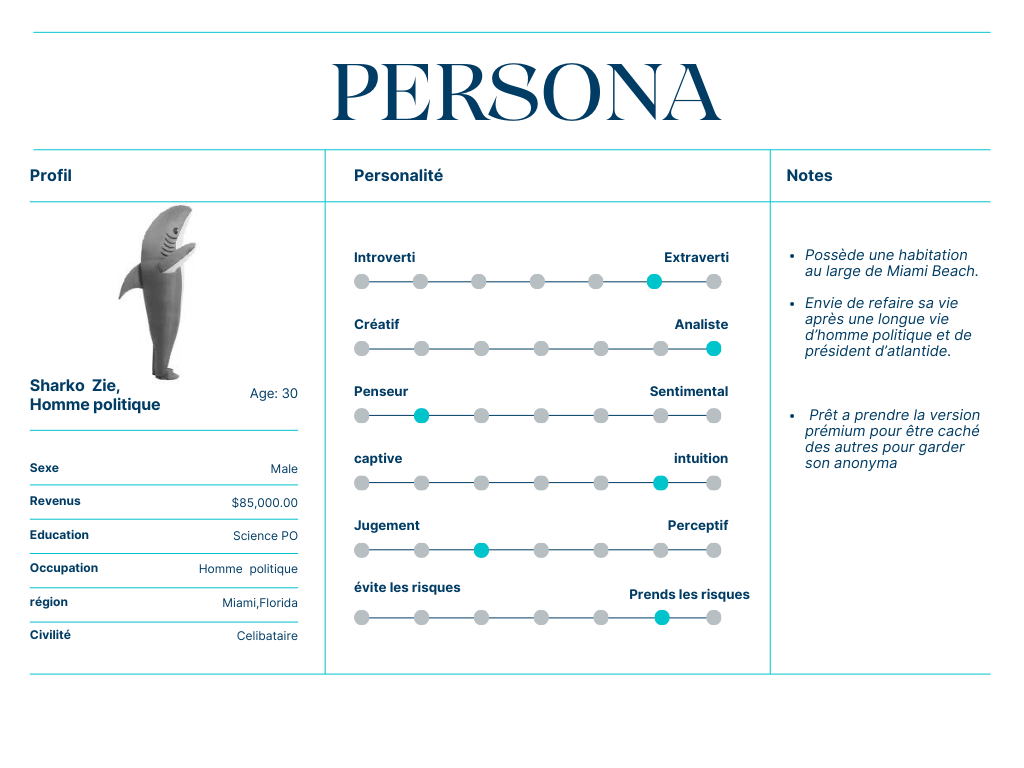
\includegraphics[width=1\textwidth]{photo/Personna_Sharkozie.png}\\

Sharko Zie, un ancien président, est un utilisateur potentiel attiré par les fonctionnalités d'anonymat offertes par l'application. 
La possibilité de masquer son identité et de modifier sa localisation grâce au mode premium répond à son besoin de discrétion. 
Ces fonctionnalités sont particulièrement utiles lorsqu'il voyage, lui permettant de connecter avec de nouveaux partenaires de chasse tout en protégeant sa vie privée. \\

\subsection*{Kaan Persona : Eric l’Athlète}
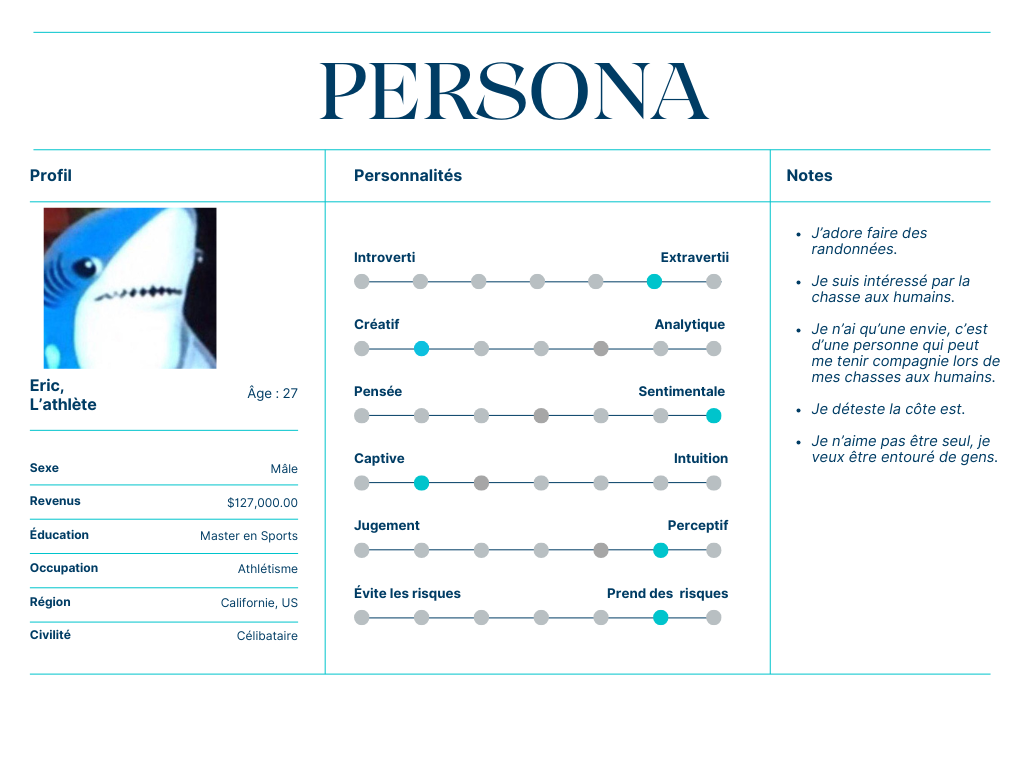
\includegraphics[width=1\textwidth]{photo/Personna_Kaan.png}\\

Eric est quelqu'un de très social qui aime avoir beaucoup d'amis et partager sa vie. Il serait un grand utilisateur des stories et des posts sur le fil d'actualité. 
Malheureusement, l'ajout d'amis est limité à un certain nombre par jour dans la version gratuite. Toutefois, la version premium offre un ajout d'amis illimité, 
ce qui conviendrait parfaitement à Eric. Par ailleurs, il n'apprécie pas la côte Est et pourrait donc utiliser le mode premium pour bloquer les utilisateurs de cette région 
et ne pas les voir sur son fil. \\

\subsection*{Nizar Persona : Bob Fisher}
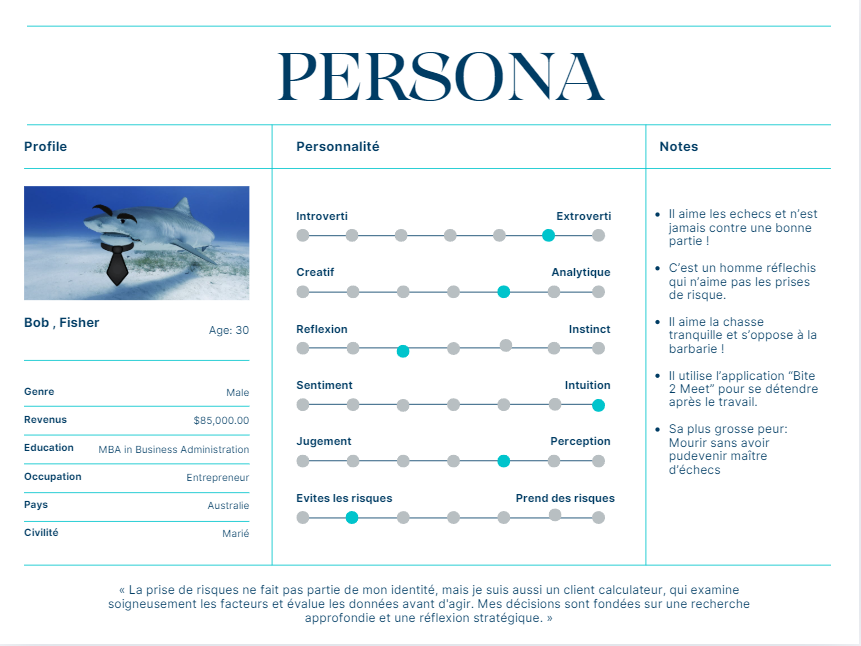
\includegraphics[width=1\textwidth]{photo/Persona_Nizar.png}\\

Bob Fisher est un entrepreneur australien passionné par les échecs. Il cherche une application qui lui permet de se détendre après le travail en organisant des sorties pour chasser
des humains , sur les plages du monde entier.\\

\section{Basse-Fidélité}
Nous avons exploré plusieurs propositions pour les versions basse-fidélité, avec des idées de différents personnes au sein du groupe et des approches variées (voir ci-dessous). 
\includegraphics[width=1\textwidth]{photo/tableau.png}
\newpage
\subsection{les différentes propositions d'idées}
\begin{figure}[H]
    \centering
    \begin{minipage}{0.4\textwidth}
        \centering
        \includegraphics[width=\linewidth]{photo/Alex_basse_fidelité.jpg}
        \caption{Idées d'Alex}
        \label{fig:Alex}
    \end{minipage}
    \hfill
    \begin{minipage}{0.4\textwidth}
        \centering
        \includegraphics[width=\linewidth]{photo/Nizar_basse_fidelité.jpg}
        \caption{Idées de Nizar}
        \label{fig:Nizar}
    \end{minipage}
    \begin{minipage}{0.4\textwidth}
        \centering
        \includegraphics[width=\linewidth]{photo/Kaan_basse_fidelité.jpg}
        \caption{Idées de Kaan (1/2)}
    \end{minipage}
    \hfill
    \begin{minipage}{0.4\textwidth}
        \centering
        \includegraphics[width=\linewidth]{photo/Kaan_basse_fidelité2.jpg}
        \caption{Idées de Kaan (2/2)}
        \label{fig:Kaan}
    \end{minipage}
\end{figure}

Ces idées, issues de nos réunions de groupe, nous ont permis de discuter de certains aspects
 de l'application, d'identifier des éléments clés à conserver, 
et de proposer des évolutions pour améliorer l'expérience utilisateur générale. \\

\subsection{Idées d'Alex}
Dans \hyperref[fig:Alex]{l'idées d'Alex} il propose  de faire une messagerie pour garder
 un contact avec les nouveaux .

\subsection{Idées de Nizar}
Dans \hyperref[fig:Nizar]{l'idées de Nizar} lui a propose une page de réglages permettant de modfier le profil, photos mais surtout
d'acceder au prémium et de voir les fonctionnalités possible à réaliser dans l'applis.

\subsection{Idées de Kaan}
Dans \hyperref [fig:Kaan]{l'idées de Kaan} il propose de faire une carte des follewers qui nous suivent sur l'appplis ainsi qu'un
réseau qui montre les connexions entre nos amis et les amis de nos amis . Il propose aussi un page de profil on y trouve 
les infos sur la personne les interets le pourcentage de compatibilité  le classement général de chasse . 




\includegraphics[width=0.5\textwidth]{photo/Visu_basse_fidelité.jpg}\caption{Idées générales}

\section{Data Abstraction}


\section{Task Abstraction}


\section{Conclusion}
Ce rapport présente les bases du projet, incluant la conception d'une application unique, les personas utilisateurs, et les premières itérations de design basse-fidélité. 
Grâce à l'analyse des données et à l'abstraction des tâches, nous avons pu identifier des fonctionnalités clés qui répondent aux besoins de nos utilisateurs. 
Les prochaines étapes incluront l'amélioration des prototypes, l'intégration des données, et des tests utilisateurs.

\end{document}